\question 在路由器进行互联的多个局域网的结构中,要求每个局域网( )
\par\fourch{物理层、数据链路层、网络层协议都必须相同,而高层协议可以不同}{物理层、数据链路层协议可以不同,而数据链路层以上的高层协议必须相同}{\textcolor{red}{物理层、数据链路层、网络层协议可以不同,而网络层以上的高层协议必须相同}}{物理层、数据链路层、网络层协议及高层协议都可以不同}
\begin{solution}本层及本层以下的协议可以不同,但是高层协议必须相同。例如,在数据链路层互连,物理层协议与数据链路层协议可以不同,但是网络层及其以上协议必须相同。
\end{solution}
\question (中南大学,2007年)在计算机网络中,能将异种网络互连起来,实现不同网络协议相互转换的网络互联设备是
\par\twoch{局域网交换机}{集线器}{路由器}{\textcolor{red}{网关}}
\begin{solution}考查异构网络互联。网关是一种充当转换重任的计算机设备,在使用不同的通信协议、数据格式或语言,甚至体系结构完全不同的两种系统之间,网关是一个翻译器。当中继系统是中继器或集线器,网桥或交换机,一般不称之为网络互连,因为这仅仅是把一个网络扩大了,而这仍然是一个网络。当中继系统是路由器时,它是用于网络协议同在IP下的异构网络互连。
\end{solution}
\question (山东大学)在下列网络设备中,传输延迟最大的是
\par\twoch{局域网交换机}{网桥}{\textcolor{red}{路由器}}{集线器}
\begin{solution}由于路由器是网络层设备,在路由器上实现了物理层、数据链路层和网络层的功能,因此路由器的传输延迟时间是最大的。
\end{solution}
\question 某网络拓扑如下图所示,路由器R1只有到达子网192.168.1.0/24的路由。为使R1可以将IP分组正确地路由到图中所有子网,则在R1中需要增加的一条路由(目的网络,子网掩码,下一跳)是(
~)。

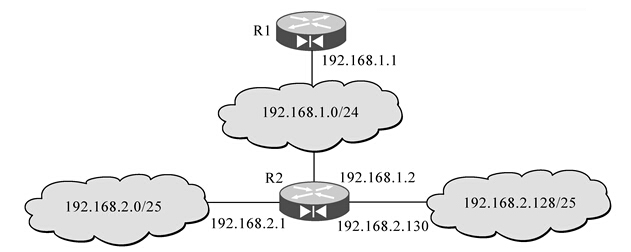
\includegraphics[width=3.33333in,height=1.33333in]{computerassets/68bb6dada2bc1a91fdc323c08ef13460.jpeg}
\par\fourch{192.168.2.0,255.255.255.128,192.168.1.1}{192.168.2.0,255.255.255.0,192.168.1.1}{192.168.2.0,255.255.255.128,192.168.1.2}{\textcolor{red}{192.168.2.0,255.255.255.0,192.168.1.2}}
\begin{solution}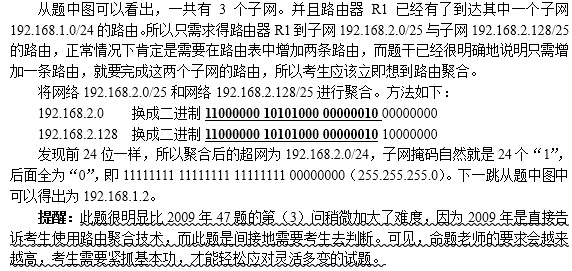
\includegraphics[width=3.33333in,height=1.58333in]{computerassets/587e0809d07702794990cae26f6745b2.jpeg}
\end{solution}
\question 下列关于IP路由器功能的描述中,正确的是( )。
\ding{192}.运行路由协议,设置路由表 \ding{193}.监测到拥塞时,合理丢弃IP分组
\ding{194}.对收到的IP分组头进行差错校验,确保传输的IP分组不丢失
\ding{195}.根据收到的IP分组的目的IP地址,将其转发到合适的输出线路上
\par\twoch{仅\ding{194}、\ding{195}}{仅\ding{192}、\ding{193}、\ding{194}}{\textcolor{red}{仅\ding{192}、\ding{193}、\ding{195}}}{\ding{192}、\ding{193}、\ding{194}、\ding{195}}
\begin{solution}\ding{192}:路由器上都会运行相应的路由协议,如RIP、OSPF协议等。另外,设置路由表也是路由器必须完成的,故\ding{192}正确。
\ding{193}:当监测到拥塞时,路由器会将IP分组丢弃,并向源点发送源抑制报文,故\ding{193}正确。
\ding{194}:尽管路由器会对IP分组首部进行差错校验,但是不能确保传输的IP分组不丢失。当路由器收到的数据报的首部中有的字段值不正确时,就丢弃该数据报,并向源站发送参数问题报文,故\ding{194}错误。
\ding{195}:这个是路由表最基本的路由功能,当路由器某个输入端口收到分组,路由器将按照分组要去的目的地(即目的网络),把该分组从路由器的某个合适的输出端口转发给下一跳路由器。下一跳路由器也按照这种方法处理分组,直到该分组到达终点为止,故\ding{195}正确。
\end{solution}
